\documentclass[oneside, 12pt]{book}
\usepackage[polish]{babel}
\usepackage{geometry}
\usepackage{lipsum}
\usepackage{nameref}
\usepackage{polski}
\usepackage[utf8]{inputenc}
\usepackage{setspace}
\usepackage[export]{adjustbox}
\usepackage{biblatex}
\usepackage{titlesec}
\usepackage{csquotes}
\usepackage[pdfsubject={Nazwisko I.: Tytuł pracy},
pdfauthor={Nazwisko I.},
pdftitle={Nazwisko I.: Tytuł pracy},
pdfkeywords={słowo kluczowe1; słowo kluczowe2; słowo kluczowe3}]{hyperref}


\setcounter{tocdepth}{3}
\setcounter{secnumdepth}{3}

\addbibresource{bibliography.bib}

\titleformat{\chapter}[block]
  {\normalfont\huge\bfseries}{\thechapter.}{1em}{\Huge}

\titlespacing*{\chapter}{0pt}{50pt}{40pt}

\geometry{
    top=1in,
    bottom=1in,
    outer=1in,
    inner=1in,
}

\pagestyle{plain} %Numeracja na dole

\linespread{1.5} % Interlinia 1.5

\setlength{\parindent}{1.25cm} % Wcięcie akapitu 1.25cm

\begin{document}
\thispagestyle{empty}

% Informacje na stronę tytułową
\newcommand{\autor}{\fontfamily{qhv}\fontshape{n}\selectfont\LARGE\bfseries
Krystian Pielat}
%
\newcommand{\album}{\fontfamily{qhv}\fontshape{n}\selectfont
143007}

\newcommand{\pltitle}{\fontfamily{qhv}\fontshape{n}\selectfont\Large\bfseries
Analiza wpływu parametrów akustycznych i tekstów na charakterystykę utworów muzycznych z wykorzystaniem metod sztucznej inteligencji}
\newcommand{\engtitle}{\fontfamily{qhv}\fontshape{n}\selectfont\Large\bfseries
 Analysis of the Influence of Acoustic Parameters and Lyrics on the Characteristics of Music Tracks Using AI Methods}
\newcommand{\level}{\fontfamily{qhv}\fontshape{n}\selectfont\Large
inżynierska} %jeśli magisterka to trzeba sobie przystosować pamiętając o specjalności
\newcommand{\kierunek}{\fontfamily{qhv}\fontshape{n}\selectfont\Large
Informatyka}
%
\newcommand{\promotor}{\fontfamily{qhv}\fontshape{n}\selectfont\large\bfseries
dr inż. Daniela Grzonki}
\newcommand{\spec}{\fontfamily{qhv}\fontshape{n}\selectfont\Large\bfseries
Brak}
\newcommand{\rok}{\fontfamily{qhv}\fontshape{n}\selectfont
2024}

% Strona tytułowa
\begin{titlepage}
\thispagestyle{empty}
\vspace*{1ex}
\fontfamily{qhv}\fontshape{n}\selectfont
\hspace{-3.5em}\parbox{0.15\textwidth}{
\includegraphics[height=0.15\textwidth]{logo_pk/logoPK.png}}
\parbox[c]{0.7\textwidth}
{\centering
\Large
{\bfseries Politechnika Krakowska}\\
{\bfseries im. Tadeusza Kościuszki}\\

\smallskip

\Large Wydział Informatyki i Telekomunikacji}\hspace{0.3em}
 \parbox{0.2\textwidth}{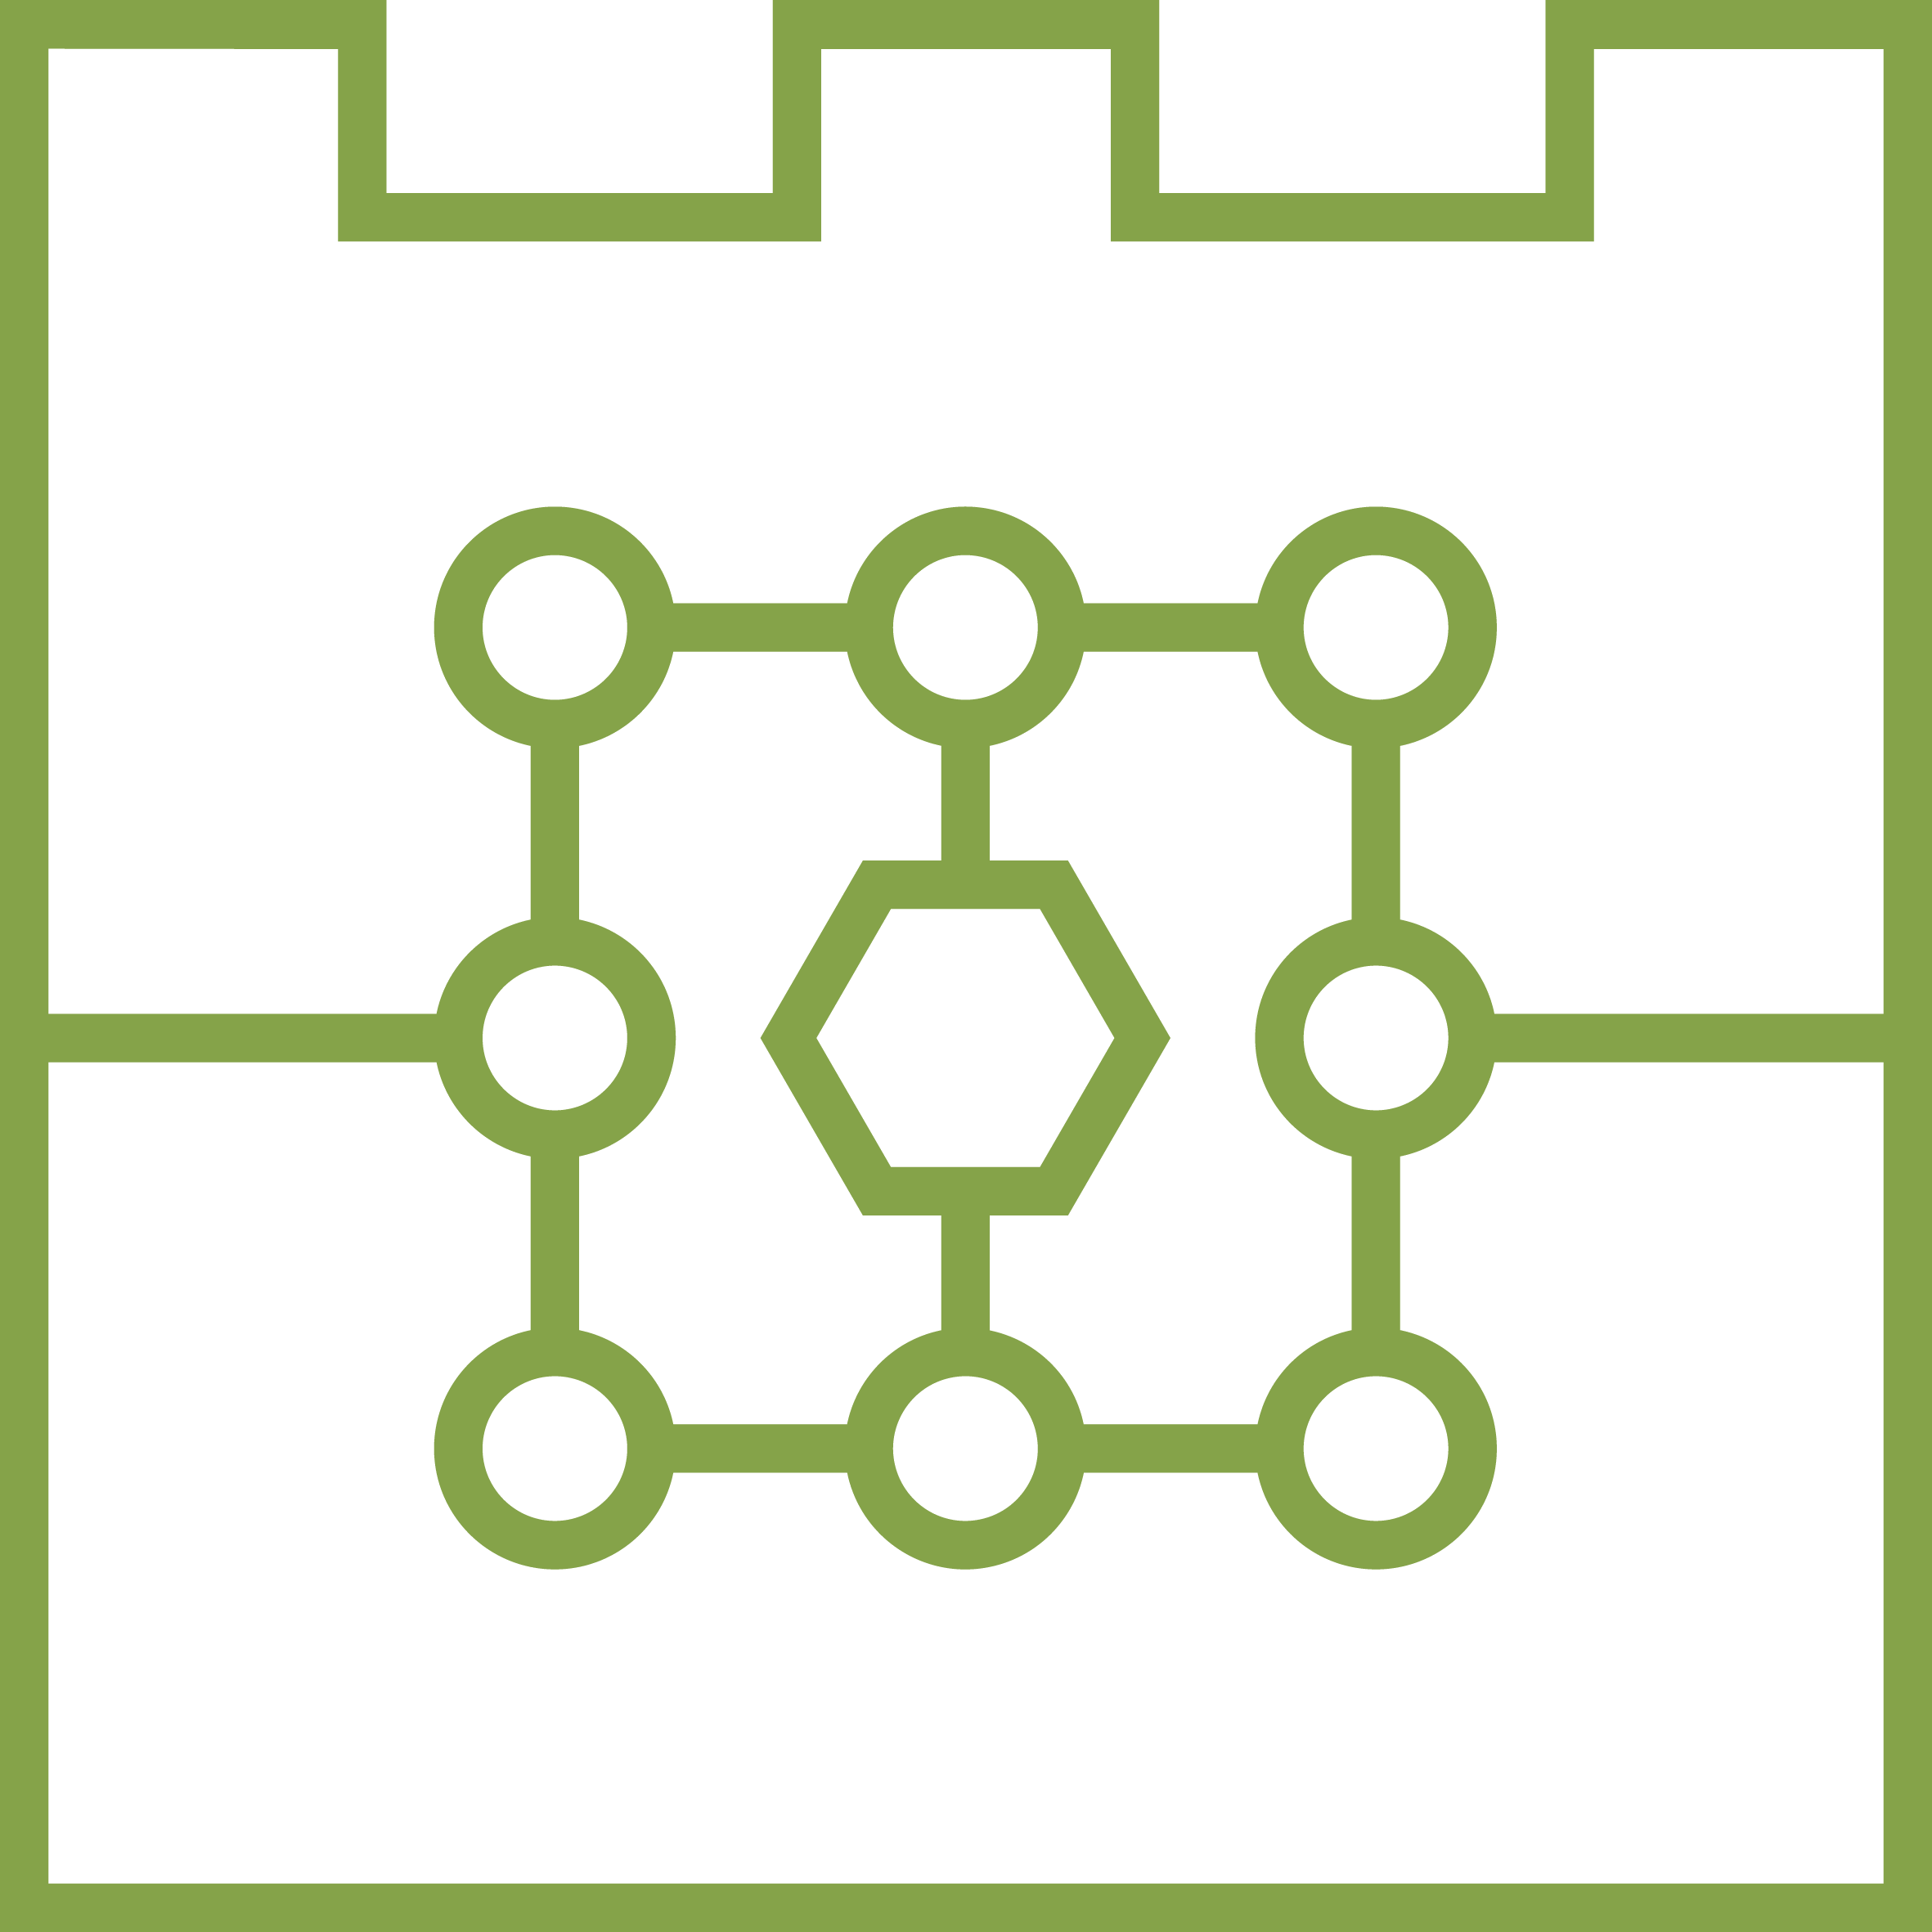
\includegraphics[width=0.15\textwidth]{logo_pk/logoIT.png}}%\hspace{0.12em}
\parbox[c]{0.15\textwidth}



 \vspace{0.10\textheight}

 \center{\autor}
 \smallskip
 \center{\large numer albumu: \album}

\vspace*{2ex}

 \center{\pltitle}

 \smallskip

 \center{\engtitle}

 \bigskip

 \center{\Large\bfseries Praca \level \\[0.2ex] %jeśli magisterka to trzeba sobie przystosować pamiętając o specjalności
\fontfamily{qhv}\fontshape{n}\selectfont\Large\bfseries na kierunku
 \kierunek\\[0.2ex]
 }

\vspace{0.11\textheight}

\hspace{0.57\textwidth} \parbox{0.42\textwidth}{Praca przygotowana pod
kierunkiem:
\\
%
\bfseries \promotor}

\vfill

 % wpisać rok
 \center{Kraków, \rok}
 \end{titlepage}

 \newpage

% \vspace*{17cm}
% \begin{flushright}
% \textit{Tu można sobie coś wpisać}
% \end{flushright}




\tableofcontents
\clearpage

\chapter{Rozdział 1}
\label{cha:rozdzial1}

\section{Podrozdział 1}
\label{sec:podrozdzial1}
Lorem ipsum dolor sit amet, consectetur adipiscing elit, sed do eiusmod tempor incididunt ut labore et dolore magna aliqua. Ut enim ad minim veniam, quis nostrud exercitation ullamco laboris nisi ut aliquip ex ea commodo consequat. Duis aute irure dolor in reprehenderit in voluptate velit esse cillum dolore eu fugiat nulla pariatur. Excepteur sint occaecat cupidatat non proident, sunt in culpa qui officia deserunt mollit anim id est laborum. \cite{stats_adoption}

\begin{center}
\begin{figure}[ht]
  
\includegraphics[width=6in]{img/plik.png}
  \caption{Podpis pod rysunkiem\cite{nature_behavior}.}
  \label{Figure:fig_beh}
\end{figure}
\end{center}

%---------------------------------------------------------------------------

\section{Podrozdział 2}
\label{sec:podrozdzial2}
Lorem ipsum dolor sit amet, consectetur adipiscing elit, sed do eiusmod tempor incididunt ut labore et dolore magna aliqua. Ut enim ad minim veniam, quis nostrud exercitation ullamco laboris nisi ut aliquip ex ea commodo consequat. Duis aute irure dolor in reprehenderit in voluptate velit esse cillum dolore eu fugiat nulla pariatur. Excepteur sint occaecat cupidatat non proident, sunt in culpa qui officia deserunt mollit anim id est laborum. \cite{norman2013design}
% \include{rozdzial2}
% \include{rozdzial3}
% \include{rozdzial4}
% \include{rozdzial5}
% \include{rozdzial6}
% \include{rozdzial7}
% \include{rozdzial8}
% \include{rozdzial9}

\cleardoublepage % Dodaj nową stronę, aby "Literatura" zaczęła się na nieparzystej stronie
\phantomsection % Dodaj punkt w spisie treści dla sekcji "Literatura"
\addcontentsline{toc}{chapter}{Bibliografia} % Dodaj "Literatura" do spisu treści, bez numerowania
\printbibliography[title={Bibliografia}]
\end{document}
